\section{Первая лабораторная работа}


\subsection{Постановка задачи}
1)Провести \textbf{анализ сетевой конфигурации} ОС (сетевые интерфейсы, назначение имеющихся сетевых интерфейсов, параметры имеющихся сетевых интерфейсов).\\
2)Найти назначение команды \textbf{ping} используя команду man или с помощью сети интернет, найти ключи команды ping, протестировать несколько найденных ключей, тестируя ключи провести анализ возможностей.\\
3)Установить базу данных \textbf{MariaDB}, настроить её, установить её в автозагрузку.\\ 
4)Установить \textbf{Apache}, настроить и добавить его в автозагрузку и проверить его работу.\\ 
5)Установить, настроить и запустить \textbf{FTP-сервер}.\\ 
6)Создать пользователя, обеспечить подключение к нему через \textbf{SSH} через логин и пароль.

\subsection{Реализация}

\subsubsection{Ход выполнения задачи №1}

\paragraph{Выведем список сетевых интерфейсов, выполнив команду \textbf{ifconfig}:}

\begin{code}
	\inputminted[breaklines=true, xleftmargin=1em, linenos, frame=single, framesep=10pt, fontsize=\footnotesize, firstline=1, lastline=33]{haskell}{fig/ifconfig1.bash}
	\caption{Информация о сетевых интерфейсах }
\end{code}

\paragraph{Исследуем два сетевых интерфейса:}
\subparagraph{lo:\\}
Интерфейс lo - это локальная петля, которая имеет IP-адрес 127.0.0.1 и предназначена для сетевого доступа к своему же компьютеру. Любые сообщения, посылаемые на этот канал, немедленно принимаются тем же самым каналом. Любые сообщения, которые отправляются с этого интерфейса, но у которых адрес не Loopback Interface, отбрасываются.\\ 
1)P-адрес (ipv4) - 127.0.0.1 он фиксированный и изменению не подлежит.\\ 
2)Маска подсети — 255.0.0.0\\
3) IP-адрес (ipv6) - ::1\\
4) MTU(Максимальный размер полезного блока данных одного пакета , который может быть передан протоколом без фрагментации) равен 65536 байт.\\
5)Информация о числе полученных, отправленных, потерянных пакетах (а также 	их объеме), ошибок и т. д.
\subparagraph{wlp1s0:\\}
Интерфейс wlp1s0 является беспроводным и обладает следующими характеристиками:
1) Максимальный размер полезного блока данных одного пакета, который может быть передан протоколом без фрагментации(MTU) равен 1500 байт.\\
2) Включён (UP), принимает широковещательные пакеты (BROADCAST), принимает групповые пакеты (MULTICAST).\\
3) IP-адрес (ipv4) - 192.168.1.4\\
4) Маска подсети - 255.255.255.0\\
5) IP-адрес (ipv6) - fe80::d877:403a:e0f9:1a30\\
6) Широковещательный адрес - 192.168.1.255\\
7) Информация о числе полученных, отправленных, потерянных пакетах (а также их объеме), ошибок и т.д.

\subsubsection{Ход выполнения задачи №2}

\paragraph{Найдем в консоли назначение команды ping с помощью команды man:\\}

Из информации полученной командой \textbf{man} следует, что команда \textbf{ping} передает небольшой пакет с данными ICMP и ожидает получить обратно пакет ответа, если получает, то считается что удаленный узел доступен. ICMP или Internet Control Message Protocol(надстройка над протоколом IP, которая используется для передачи служебных сообщений и сообщений об ошибках) может передавать только два типа пакетов - это сообщения с отчетами и сообщения запросов. В свою очередь, сообщения запросов делятся на эхо-запрос и эхо-ответ.

\paragraph{Найдем в консоли назначение ключей команды ping с помощью команды man:\\}

\textbf{-4} — Использует только IPv4(по умолчанию).\\
\textbf{-6} — Использует только IPv6.\\
\textbf{-a} — Сигнализирует о возвращении пакета с помощью динамика.\\
\textbf{-А} — В чрезвычайно плохих сетевых условиях мог выйти новый запрос, прежде чем последний возвращен. Новый запрос звона выходит, как только последний ответ получен.\\
\textbf{-b} — Разрешает отправлять пакеты на широковещательный адрес.\\
\textbf{-c} (count) — Останавливается после отправки указанного в аргументе кол-ва пакетов.\\

\begin{code}
	\inputminted[breaklines=true, xleftmargin=1em, linenos, frame=single, framesep=10pt, fontsize=\footnotesize, firstline=1, lastline=33]{haskell}{fig/ping-c.bash}
	\caption{Результат работы команды \textbf{ping} с ключом \textbf{-c}}
\end{code}

\newpage

\textbf{-D} — выводить время в виде UNIX timestamp.\\

\begin{code}
	\inputminted[breaklines=true, xleftmargin=1em, linenos, frame=single, framesep=10pt, fontsize=\footnotesize, firstline=1, lastline=33]{haskell}{fig/ping-D.bash}
	\caption{Результат работы команды \textbf{ping} с ключом \textbf{-D}}
\end{code}

\textbf{Unix Timestamp} – это метка времени, которая представляет собой последовательность символов, отражающих количество секунд, прошедших с 1 января 1970 года.\\ 
\textbf{-f} — Отправка пакетов без задержки. При отправке пакета печатается ".". Если приходит ответ, то "." удаляется. Может использоваться только суперпользователем.\\
\textbf{-h} — Справка.\\
\textbf{-i} — Выдерживает интервал между отправкой пакетов, задаваемый в аргументе. Только суперпользователь может указать интервал меньше 0.2.\\
\textbf{-w}(deadline) — Указывается максимальное время ожидания возвращения пакета(миллисекунды).\\
\textbf{-M} — Если нужно найти самый подходящий размер MTU с помощью команды Ping, следует определить начальное значение и уменьшать его до тех пор, пока прекратятся ошибки.\\ 
MTU (Maximum Transmission Unit) это максимальный размер пакета, который может быть передан по сети без фрагментации.\\
\textbf{-q} — Не выводится ничего кроме строки в начале и итоговой информации в конце.\\ 
\textbf{-s} — В аргументе задаётся размер передаваемых пакетов.

\begin{code}
	\inputminted[breaklines=true, xleftmargin=1em, linenos, frame=single, framesep=10pt, fontsize=\footnotesize, firstline=1, lastline=33]{haskell}{fig/ping-s.bash}
	\caption{Результат работы команды \textbf{ping} с ключом \textbf{-s}}
\end{code}

\subsubsection{Ход выполнения задачи №3}

\paragraph{Установим MariaDB и проверим работает ли база данных:}

\begin{code}
	\inputminted[breaklines=true, xleftmargin=1em, linenos, frame=single, framesep=10pt, fontsize=\footnotesize, firstline=1, lastline=33]{haskell}{fig/mariadb.bash}
	\caption{Вывод статуса базу данных}
\end{code}

\paragraph{Настроем базу данных для обеспечения её безопасности.}

\paragraph{Добавим БД в автозагрузку:}

\begin{code}
	\inputminted[breaklines=true, xleftmargin=1em, linenos, frame=single, framesep=10pt, fontsize=\footnotesize, firstline=1, lastline=33]{haskell}{fig/database.bash}
	\caption{Результат добавления БД в автозагрузку}
\end{code}

\subsubsection{Ход выполнения задачи №4}

\paragraph{Установим apache2 с помощью следующей команды:}

\begin{code}
	\inputminted[breaklines=true, xleftmargin=1em, linenos, frame=single, framesep=10pt, fontsize=\footnotesize, firstline=1, lastline=33]{haskell}{fig/apache2.bash}
	\caption{Команда для установки apache2}
\end{code}

\paragraph{Выведем список правил брандмауэра, чтобы проверить, нужна ли их настройка:}

\begin{code}
	\inputminted[breaklines=true, xleftmargin=1em, linenos, frame=single, framesep=10pt, fontsize=\footnotesize, firstline=1, lastline=33]{haskell}{fig/status.bash}
	\caption{Список правил брэндмауэра}
\end{code}

\paragraph{Включим самый ограниченный профиль, который будет позволять входящий трафик:}

\begin{code}
	\inputminted[breaklines=true, xleftmargin=1em, linenos, frame=single, framesep=10pt, fontsize=\footnotesize, firstline=1, lastline=33]{haskell}{fig/status1.bash}
	\caption{Обновление правил брэндмауэра}
\end{code}

\paragraph{Проверим, находится ли Apache2 в автозагрузке:}

\begin{code}
	\inputminted[breaklines=true, xleftmargin=1em, linenos, frame=single, framesep=10pt, fontsize=\footnotesize, firstline=1, lastline=33]{haskell}{fig/status2.bash}
	\caption{Результат вывода процессов, которые находятся в автозагрузке}
\end{code}


\paragraph{Запустим наш сервер и проверим, работает ли он:}

\begin{code}
	\inputminted[breaklines=true, xleftmargin=1em, linenos, frame=single, framesep=10pt, fontsize=\footnotesize, firstline=1, lastline=33]{haskell}{fig/apache2sys.txt}
	\caption{Вывод статуса сервера Apache2}
\end{code}

\subsubsection{Ход выполнения задачи №5}

\paragraph{Установим FTP-server следующей командой:}

\begin{code}
	\inputminted[breaklines=true, xleftmargin=1em, linenos, frame=single, framesep=10pt, fontsize=\footnotesize, firstline=1, lastline=33]{haskell}{fig/install_vsftpd.txt}
	\caption{Команда, введеная в консоли}
\end{code}

\newpage

\paragraph{Откроем порты 20 и 21 для нормальной работы FTP сервера:}

\begin{code}
	\inputminted[breaklines=true, xleftmargin=1em, linenos, frame=single, framesep=10pt, fontsize=\footnotesize, firstline=1, lastline=33]{haskell}{fig/vsftpd_ports.bash}
	\caption{Команды, введеные в консоли}
\end{code}

\paragraph{Включим FTP сервер и добавим его в автозагрузку:}

\begin{code}
	\inputminted[breaklines=true, xleftmargin=1em, linenos, frame=single, framesep=10pt, fontsize=\footnotesize, firstline=1, lastline=33]{haskell}{fig/vsftpd_enable.bash}
	\caption{Команды, введеные в консоли}
\end{code}

\paragraph{Проверим состояние FTP сервера командой \textbf{sudo systemctl status vsftpd}:}

\begin{code}
	\inputminted[breaklines=true, xleftmargin=1em, linenos, frame=single, framesep=10pt, fontsize=\footnotesize, firstline=1, lastline=33]{haskell}{fig/vsftpd_status.bash}
	\caption{Статус FTP сервера}
\end{code}

\subsubsection{Ход выполнения задачи №6}

\paragraph{Создадим пользователя и установим ему пароль.}

\paragraph{Подключимся к пользователю:}

\begin{code}
	\inputminted[breaklines=true, xleftmargin=1em, linenos, frame=single, framesep=10pt, fontsize=\footnotesize, firstline=1, lastline=33]{haskell}{fig/end.bash}
	\caption{Результат подключения}
\end{code}

\subsection{Вывод}
Мы научились выводить информацию о \textbf{сетевых интерфейсах}, исследовать их с помощью, полученной с помощью команды \textbf{ifconfig}, информации и узнали назначение сетевых интерфейсов, поднятых на ПК.\\
Мы научились работать с командой \textbf{man} и разобрались в назначении и принципе работы команды \textbf{ping}. Мы разобрались в работе нескольких ключей команды \textbf{ping} и прочитали как работают остальные. Теперь нам понятен функцонал и способы использования команды \textbf{ping}.\\
Мы научились устанавливать, настраивать и подключать базу данных \textbf{MariaDB}, а также  научились выводить список программ, находящихся в автозагрузке.\\
Мы научились устанавливать сервер \textbf{Apache2}, работать с правилами брандмауэра, запускать веб-сервер и проверять его работоспособность.\\
Мы научились устанавливать, настраивать и запускать \textbf{FTP сервер}.\\
Мы научились создавать пользователей в системе и обеспечивать подключение к ним через \textbf{SSH} с использованием логина и пароля.

\newpage

\section{Вторая лабораторная работа}

\subsection{Постновка задачи}
С помощью доступных материалов разобраться в технологии \textbf{Ethernet}. Найти и
описать \textbf{стандарты Ethernet}. Описать \textbf{Ethernet-фреймы}. Установить утилиту \textbf{Wireshark}. Проанализировать с ее помощью Ethernet заголовок одного из сгенерированных командой ping пакетов.

\subsection{Реализация}

\subsubsection{Теоретическая информация\cite{Ethernetfr}\cite{main}\cite{StEthernet}}

\paragraph{Что такое Ethernet?}
    
Ethernet — это набор описаний способов физической передачи сигналов (первоначально по коаксиальному кабелю) на первом уровне модели OSI (физический) и формирования кадров (фреймов) на втором уровне модели OSI (канальный) внутри локальных сетей LAN. 


\paragraph{Какие стандарты Ethernet существуют и какие у них характеристики?}

(Число 10 обозначает номинальную битовую скорость передачи данных стандарта, то есть 10Мбит/с а слово «Base» - метод передачи на одной базовой частоте. Последний символ обозначает тип кабеля.)
    
\begin{itemize}
    \item 10Base-5 - коаксиальный кабель диаметром 0,5 дюйма (1дм=2,54см), называемый «толстым» коаксиальным кабелем, с волновым сопротивлением 50Ом. используется как моноканал для всех станций, максимальная длина сегмента 500м. Станция подключаться к кабелю через приемопередатчик - трансивер. Трансивер соединяется с сетевым адаптером разъема DB-15 интерфейсным кабелем AUI. Требуется наличие терминаторов на каждом конце, для поглощения распространяющихся по кабелю сигналов.
\end{itemize}
\begin{figure}[H]
	\begin{center}
		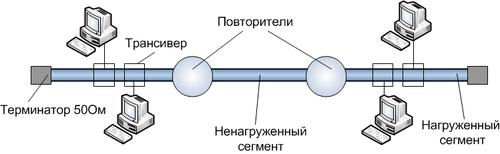
\includegraphics[scale=0.7]{fig/10Base-5.png}
		\caption{Стандарт 10Base-5}
		\label{pic:10Base-5} % название для ссылок внутри кода
	\end{center}
\end{figure}

\begin{itemize}
        \item 10Base-2 - коаксиальный кабель диаметром 0,25 дюйма, называемый «тонким» коаксиальным кабелем, с волновым сопротивлением 50Ом. Используется как моноканал для всех станций, максимальная длина сегмента 185 м. Для подключения кабеля к сетевой карте нужен T-коннектор, а на кабеле должен быть BNC-коннектор.
\end{itemize}
\begin{figure}[H]
	\begin{center}
	    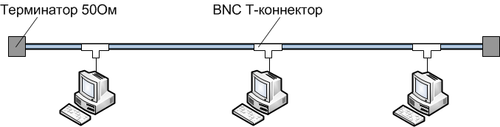
\includegraphics[scale=0.7]{fig/10Base-2.png}
        \caption{Стандарт 10Base-2}
	    \label{pic:10Base-2} % название для ссылок внутри кода
    \end{center}
\end{figure}  

\noindent(Стандарт сетей на коаксиальном кабеле разрешает использование в сети не более 4 повторителей и, соответственно, не более 5 сегментов кабеля. При максимальной длине сегмента кабеля в 500 м это дает максимальную длину сети в 500*5=2500 м. Только 3 сегмента из 5 могут быть нагруженными, то есть такими, к которым подключаются конечные узлы. Между нагруженными сегментами должны быть ненагруженные сегменты.)

\begin{itemize}
\item 10Base-T - кабель на основе неэкранированной витой пары (Unshielded Twisted Pair, UTP). Образует звездообразную топологию на основе концентратора, концентратор осуществляет функцию повторителя и образует единый моноканал, максимальная длина сегмента 100м. Конечные узлы соединяются с помощью двух витых пар. Одна пара для передачи данных от узла к концентратору - Tx, а другая для передачи данных от концентратора к узлу – Rx.
\end{itemize}
\begin{figure}[H]
    \begin{center}
	    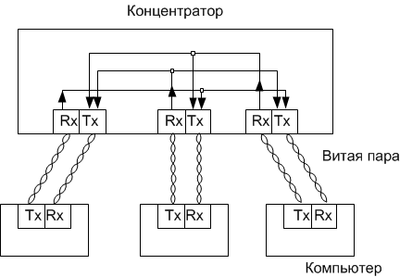
\includegraphics[scale=0.7]{fig/10Base-T.png}
	    \caption{Стандарт 10Base-T}
	    \label{pic:10Base-T} % название для ссылок внутри кода
    \end{center}
\end{figure}
    
\noindent(В стандарте сетей на витой паре определено максимально число концентраторов между любыми двумя станциями сети, а именно 4.)

\begin{itemize}
\item 10Base-F - волоконно-оптический кабель. Функционально сеть Ethernet на
оптическом кабеле состоит из тех же элементов, что и сеть стандарта 10Base- T. Стандарт FOIRL (Fiber Optic Inter-Repeater Link) первый стандарт комитета
802.3 для использования оптоволокна в сетях Ethernet. Мах длина сегмента 1000м, мах число хабов 4, при общей длине сети не более 2500 м.
\end{itemize}
\begin{figure}[H]
    \begin{center}
	    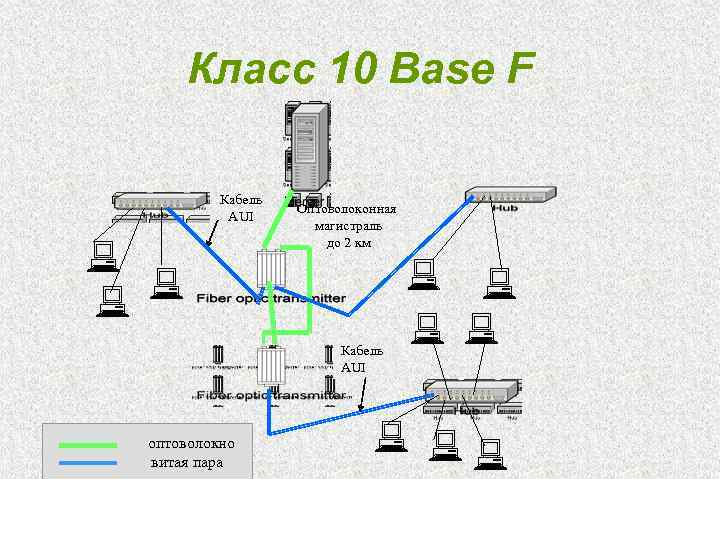
\includegraphics[scale=0.5]{fig/10Base-F.png}
	    \caption{Стандарт 10Base-F}
	    \label{pic:10Base-F} % название для ссылок внутри кода
    \end{center}
\end{figure}

\paragraph{Какие существуют Ethernet-фреймы и какие у них характеристики?}

\begin{itemize}
    \item \textbf{Xerox Ethernet}\\
Технология, основанная на коаксиальном кабеле с максимальной скоростью 3 мегабита в секунду. Модификация StarLan, в которой впервые была применена витая пара. Скорость такого соединения невелика – всего 1 мегабит в секунду.
    
    \item \textbf{Ethernet II (Ethernet DIX)}\\ 
Фирменный стандарт Ethernet компании Xerox, Intel, DEC. Все компьютеры сети подключались к общему коаксиальному кабелю. Коаксиальный кабель (coaxial, от co — совместно и axis — ось, то есть «соосный») – это кабель из пары проводников – центрального провода и окружающего его металлического цилиндра – экрана. Промежуток между проводом и экраном заполнен изоляцией, снаружи кабель так же покрыт изолирующей оболочкой. Такой кабель используется, например, в телевизионных антеннах.
    
    \item \textbf{IEEE 802.3}\\ 
    Юридический стандарт Ethernet. 
\end{itemize}    
\noindent(Ethernet II и IEEE 802.3 незначительно отличаются. Первый из них исторически раньше появился и при появлении второго много оборудования было на Ethernet II. Сейчас поддерживаются оба. Различие в том, что в Ethernet II передавался тип протокола, а по IEEE 802.3 вместо него передавалась длина поля данных.)

\newpage

\subsubsection{Ход выполнения работы}

\paragraph{Установим утилиту Wireshark с помощью следующих команд:}

\begin{code}
	\inputminted[breaklines=true, xleftmargin=1em, linenos, frame=single, framesep=10pt, fontsize=\footnotesize, firstline=1, lastline=33]{haskell}{fig/wireshark.bash}
	\caption{Команды, введенные в консоли}
\end{code}

\paragraph{Откроем утилиту Wireshark и проанализируем трафик проходящий через Ethernet интерфейс (enxd0374516eb73)}

\begin{itemize}
    \item Сгенерируем трафик с помощью команды ping, отправив 1 пакет на плоский адрес ya.ru:
\begin{code}
	\inputminted[breaklines=true, xleftmargin=1em, linenos, frame=single, framesep=10pt, fontsize=\footnotesize, firstline=1, lastline=33]{haskell}{fig/ping.bash}
	\caption{Результат работы команды \textbf{ping}}
\end{code}

    \item Проанализируем Ethernet заголовок пакета, полученного утилитой \textbf{Wireshark}:

\begin{code}
	\inputminted[breaklines=true, xleftmargin=1em, linenos, frame=single, framesep=10pt, fontsize=\footnotesize, firstline=1, lastline=33]{haskell}{fig/packet.bash}
	\caption{Характеристики пакета}
\end{code}

\end{itemize}

\newpage

1)Информация о пункте назначения(Название устрйоства, IPv4 и IPv6 адрес)\\
2)Информация о источнике(Название устрйоства, IPv4 и IPv6 адрес)\\
3)Версия протокола IP с помощью которого был отправлен пакет.\\
4)Информация о вспомогательном сетевом протоколе (ICMP), который использовался при передаче пакета.

\subsection{Вывод}
Мы изучили \textbf{стандарты Ethernet}, а также \textbf{Ethernet-фрэймы}. Также установили утилиту \textbf{Wireshark}. Научились пользоваться ей. Сгенерировали трафик с помощью команды \textbf{ping} и проанализировали \textbf{Ethernet заголовок} одного из сгенерированных пакетов.

\newpage

\section{Третья лабораторная работа}

\subsection{Постновка задачи}
С помощью доступных материалов разобраться в \textbf{протоколе IP}. Найти и описать
\textbf{стандарты протокола IP}. Установить утилиту \textbf{Wireshark}. Сгенерировать трафик и проанализировать \textbf{IP заголовок} одного из сгенерированных пакетов.

\subsection{Реализация}
\subsubsection{Теоретическая информация\cite{IP}}


Протокол IP объединяет сегменты сети в единую
сеть, обеспечивая доставку пакетов данных между    любыми узлами сети через произвольное число промежуточных узлов (маршрутизаторов).\\


Он классифицируется как протокол \textbf{сетевого уровня} по сетевой модели OSI.\\


IP \textbf{не гарантирует надёжной доставки пакета до адресата} — в частности, пакеты могут прийти не в том порядке, в котором были отправлены, продублироваться (приходят две копии одного пакета), оказаться повреждёнными (обычно повреждённые пакеты уничтожаются) или не прийти вовсе. Гарантию безошибочной доставки пакетов дают некоторые протоколы более высокого уровня — транспортного уровня сетевой модели OSI, — например, TCP, которые используют IP в качестве транспорта.\\


\textbf{IPv4} — четвёртая версия протокола IP.
IPv4 использует 32-битные адреса, ограничивающие адресное пространство 4 294 967 296 возможными уникальными адресами.
Традиционной формой записи IPv4 адреса является запись в виде четырёх десятичных чисел (от 0 до 255), разделенных точками. Через дробь указывается длина маски подсети.\\


\textbf{Для гибкости в назначении адресов сетей и возможности использовать большое число малых и средних сетей} адресное пространство было разделено на несколько логических групп и в каждой группе отводилось разное соотношение хостов и подсетей. Эти группы носят названия классов сетей и пронумерованы латинскими буквами: A, B, C, D и E. Деление основывается на старших битах адреса.\\


\textbf{Класс А}: 0.XXX.XXX.XXX — 127.XXX.XXX.XXX
Первый бит адреса равен нулю, таким образом, класс А \textbf{занимает половину всего адресного пространства}. Адрес сети занимает 7 бит, адрес узла — 24 бита, следовательно класс A содержит 128 подсетей по 16 777 216 адресов в каждой.\\


\textbf{Класс B}: 128.0.XXX.XXX — 191.255.XXX.XXX
Класс B \textbf{занимает четверть всего адресного пространства}. Адрес сети занимает 14 бит, адрес узла — 16, следовательно класс B содержит 16 384 подсетей по 65 536 адресов в каждой.\\


\textbf{Класс C}: 192.0.0.XXX — 223.255.255.XXX
Класс C \textbf{занимает 1/8 адресного пространства}. Адрес сети занимает 21 бит, адрес узла — 8 бит, следовательно класс C содержит 2 097 152 сетей по 256 адресов в каждой.\\


\textbf{Класс D}: 224.XXX.XXX.XXX — 239.XXX.XXX.XXX
Класс D \textbf{занимает 1/16 адресного пространства. Используется для многоадресной рассылки}.\\


\textbf{Класс Е}: 240.XXX.XXX.XXX — 255.XXX.XXX.XXX.
\textbf{Такие адреса запрещены. Зарезервировано для использования в будущем.}\\


\textbf{IPv6} — шестая версия протокола IP. Иногда утверждается, что новый протокол может обеспечить до 5·1028 адресов на каждого жителя Земли. Такое большое адресное пространство было введено ради иерархичности адресов (это упрощает маршрутизацию). Тем не менее, увеличенное пространство адресов \textbf{сделает NAT необязательным}. Классическое применение IPv6 (по сети /64 на абонента; используется только unicast- адресация) обеспечит возможность использования более 300 млн IP-адресов на каждого жителя Земли.\\


Улучшения IPv6 по сравнению с IPv4:
\begin{itemize}
    \item В сверхскоростных сетях \textbf{возможна поддержка огромных пакетов (джамбограмм)} — до 4 гигабайт;
    \item Time to Live переименовано в Hop Limit
    \item Появились метки потоков и классы трафика
    \item Появилось многоадресное вещание.
\end{itemize}


\subsubsection{Ход выполнения работы}

\paragraph{Установим утилиту Wireshark с помощью следующих команд:}

\begin{code}
	\inputminted[breaklines=true, xleftmargin=1em, linenos, frame=single, framesep=10pt, fontsize=\footnotesize, firstline=1, lastline=33]{haskell}{fig/wireshark.bash}
	\caption{Команды, введенные в консоли}
\end{code}

\newpage

\paragraph{Узнаем, пакеты с какого интерфейса нас интересуют с помощью команды ifconfig:}

\begin{code}
	\inputminted[breaklines=true, xleftmargin=1em, linenos, frame=single, framesep=10pt, fontsize=\footnotesize, firstline=1, lastline=33]{haskell}{fig/ifconfig.bash}
	\caption{Результат работы команды \textbf{ifconfig}}
\end{code}

\paragraph{Сгенерируем трафик в локальной сети с помощью команды ping:}

\begin{code}
	\inputminted[breaklines=true, xleftmargin=1em, linenos, frame=single, framesep=10pt, fontsize=\footnotesize, firstline=1, lastline=33]{haskell}{fig/ping1.bash}
	\caption{Результат работы команды \textbf{ping}}
\end{code}

\newpage

\paragraph{Выберем один из сгенерированных пакетов, проходящих через интерфейс wlp1s0, и распишем его характеристики:}

\begin{code}
	\inputminted[breaklines=true, xleftmargin=1em, linenos, frame=single, framesep=10pt, fontsize=\footnotesize, firstline=1, lastline=33]{haskell}{fig/packet1.bash}
	\caption{Характеристики пакета}
\end{code}

\noindent1) Используется протокол IPv4.\\
2) Wireshark определяет максимальное количество маршрутизаторов на пути следования пакета. Наличие этого параметра не позволяет пакету бесконечно ходить по сети.
Каждый маршрутизатор при обработке пакета должен уменьшить значение TTL на
единицу. Пакеты, время жизни которых стало равно нулю, уничтожаются, а
отправителю посылается сообщение ICMP Time Exceeded. На отправке пакетов с
разным временем жизни основана трассировка их пути прохождения (traceroute).
Максимальное значение TTL=255. Обычное начальное значение TTL=64 (зависит от
ОС). В нашем случае TTL=64.\\
3) Указано, какой сетевой протокол использует сгенерированный пакет(ICMP).\\
4) 16-битная контрольная сумма, используемая для проверки целостности заголовка. Каждый хост или маршрутизатор сравнивает контрольную сумму заголовка со
значением этого поля и отбрасывает пакет, если они не совпадают. Целостность
данных IP не проверяет — она проверяется протоколами более высоких уровней
(такими, как TCP или UDP), которые тоже используют контрольные суммы.
Поскольку TTL уменьшается на каждом шаге прохождения пакета, сумма тоже должна
вычисляться на каждом шаге. (0xb751)\\
5) 32-битный адрес отправителя пакета. Может не совпадать с настоящим адресом отправителя из-за NAT. (192.168.1.3)\\
6) 32-битный адрес получателя пакета. Также может меняться из-за NAT. (192.168.1.4) 



\subsection{Вывод}
Мы разобрались в 4 и 6 версиях \textbf{протокола IP}. Мы установили утилиту \textbf{Wireshark}. Научились пользоваться ей. Сгенерировали трафик с
помощью команды \textbf{ping} и проанализировали \textbf{IP заголовок} одного из сгенерированных пакетов.

\newpage

\section{Четвертая лабораторная работа}

\subsection{Постановка задачи}

1)С помощью доступных материалов разобраться в \textbf{протоколе DHCP}. Проанализировать \textbf{DHCP заголовок} одного из пакетов.\\
2)С помощью доступных материалов разобраться в \textbf{протоколе TCP}. Проанализировать \textbf{TCP заголовок} одного из пакетов.\\
3)С помощью доступных материалов разобраться в \textbf{протоколе UDP}. Проанализировать \textbf{UDP заголовок} одного из пакетов.

\subsection{Реализация}

\subsubsection{Ход выполнения задачи №1}

\paragraph{Теоретическая информация:\cite{DHCP}\\}

\textbf{DHCP}(протокол динамической настройки узла) — сетевой протокол, позволяющий компьютерам автоматически получать IP-адрес и другие параметры, необходимые для работы в сети.\\


\textbf{Цель DHCP} — устранить два основных ограничения, накладывающихся на другие анагологичные протоколы, а именно: отсутствие поддержки динамического назначения IP-адресов и возможность передавать от сервера на станцию-клиент лишь небольшое число параметров конфигурации.\\


В \textbf{роли транспортного протокола} для обмена DHCP-сообщениями выступает \textbf{UDP}.\\


\textbf{При отправке сообщения с клиента на сервер} используется 67-й порт DHCP-сервера. При передаче в обратном направлении - 68-й.\\


\textbf{Алгоритм работы}:
\begin{itemize}
    \item Клиент посылает в свою подсеть широковещательное сообщение \textbf{DHCPDISCOVER}, в котором могут указываться устраивающие клиента IP-адрес и срок его аренды. В качестве IP-адреса источника указывается 0.0.0.0, в качестве адреса назначения - 255.255.255.255. Если DHCP-сервер отсутствует в подсети, то \textbf{сообщение будет передано в другие подсети} агентами протокола BOOTP.
    \item \textbf{Получив запрос от клиента}, DHCP-сервер отвечает на него сообщением \textbf{DHCPOFFER}. В сообщение включается предлагаемый IP-адрес (yiaddr) и прочие конфигурации для клиента (адреса маршрутизаторов, DNS-серверов и т.д.). (На данном этапе сервер не обязан резервировать адрес, который он отправил клиенту)
    \item \textbf{Получив конфигурации от серверов} (их может быть несколько, если в подсети более одного DHCP-севрера), клиент отправляет \textbf{широковещательное сообщение DHCPREQUEST}. В нем содержатся идентификатор выбранного сервера и, возможно, желательные значения запрашиваемых параметров конфигурации.(На данном этапе допускается, что клиента не устроит ни один из предложенных адресов, тогда он вновь отправит \textbf{DHCPDISCOVER})
    \item  \textbf{Получив DHCPREQUEST и убедившись, что в сообщении его идентификатор}, сервер проверяет свободен ли в данный момент запрошенный адрес. Если да, то отправляет \textbf{DHCPACK} и вносит запись в базу, иначе отправляет \textbf{DHCPNACK}.
    \item \textbf{Получив сообщение DHCPACK}, клиент обязан убедиться в уникальности IP-адреса (средствами протокола ARP) и зафиксировать суммарный срок его аренды.(Время, прошедшее между отправкой сообщения \textbf{DHCPREQUEST} и приемом ответного сообщения \textbf{DHCPACK} + срок аренды, указанный в \textbf{DHCPACK}.
    Если адрес уже используется другой станцией, клиент отправляет \textbf{DHCPDECLINE} и начинает всю процедуру снова.)
    \item Для досрочного прекращения аренды адреса клиент отправляет серверу сообщение \textbf{DHCPRELEASE}.\\
\end{itemize}


\textbf{Заголовок DHCP пакета:}
\begin{itemize}
    \item \textbf{op}
    Тип сообщения (1 = BOOTREQUEST, 2 = BOOTREPLY)
    \item \textbf{htype}
    Тип адреса оборудования
    \item \textbf{hlen}
    Длина адреса оборудования
    \item \textbf{hops}
    Используется ретранслирующим агентом
    \item \textbf{xid}
    Идентификатор транзакции между сервером и клиентом
    \item \textbf{secs}
    Время с момента выдачи DHCPREQUEST или начала обновления конфигурации
    \item \textbf{flags}
    Флаги (первый бит маркирует широковещательные сообщения)
    \item \textbf{ciaddr}
    IP-адрес клиента
    \item \textbf{yiaddr}
    <Ваш> (клиентский) IP-адрес
    \item \textbf{siaddr}
    IP-адрес следующего сервера, участвующего в загрузке
    \item \textbf{giaddr}
    IP-адрес ретранслирующего агента
    \item \textbf{chaddr}
    <Аппаратный> адрес клиента
    \item \textbf{sname}
    Хост-имя сервера (опция)
    \item \textbf{file}
    Имя загрузочного файла
    \item \textbf{options}
    Поле дополнительных параметров
\end{itemize}


\paragraph{Ход выполнения работы:}
\begin{itemize}
    \item Установим утилиту DHCPING c помощью следующей команды:
    \begin{code}
	\inputminted[breaklines=true, xleftmargin=1em, linenos, frame=single, framesep=10pt, fontsize=\footnotesize, firstline=1, lastline=33]{haskell}{fig/dhcping.bash}
	\caption{Команда, введёная в консоли}
    \end{code}
    (Утилита DHCPING проверяет DHCP-сервер используя unicast пакеты.)
    \item Для того чтобы найти IP адрес DHCP-сервера воспользуемся следующей командой: 
    \begin{code}
	\inputminted[breaklines=true, xleftmargin=1em, linenos, frame=single, framesep=10pt, fontsize=\footnotesize, firstline=1, lastline=33]{haskell}{fig/dhcp_serv.bash}
	\caption{Команда, введёная в консоли}
    \end{code}
    \item После того как мы получили ответ с IP адреса 192.168.0.1 отправим на него пакет используя следующую команду:
    \begin{code}
	\inputminted[breaklines=true, xleftmargin=1em, linenos, frame=single, framesep=10pt, fontsize=\footnotesize, firstline=1, lastline=33]{haskell}{fig/dhcp_serv1.bash}
	\caption{Команда, введёная в консоли}
    \end{code}
    
    
    
    \item Сгенерируем трафик с помощью утилиты dhcping
    \begin{figure}[H]
    \begin{center}
	    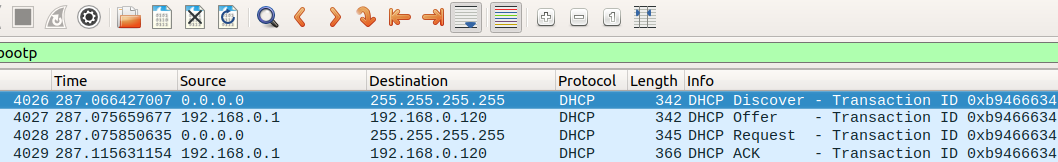
\includegraphics[scale=0.7]{fig/dhcping.png}
	    \caption{Сгенерированные пакеты}
	    \label{pic:10dadwad} % название для ссылок внутри кода
    \end{center}
    \end{figure}
    
    \newpage
    
    \item Поочерёдно проанализируем четыре пакета:
    \begin{itemize}
        \item \textbf{DHCP Discover}\\
        
        
        \begin{code}
	    \inputminted[breaklines=true, xleftmargin=1em, linenos, frame=single, framesep=10pt, fontsize=\footnotesize, firstline=1, lastline=33]{haskell}{fig/discover.bash}
	    \caption{DHCP(Discover) заголовок пакета}
        \end{code}

    1)Тип сообщения: BOOTREQUEST\\
    
    
    2)Тип адреса оборудования: Ethernet\\
    
    
    3)Длина адреса оборудования: 6 байт\\
    
    
    4)Не используется ретранслирующим агентом\\
    
    
    5)Индентификатор транзакции между сервером и клентом: 0xb9466634\\
    
    
    6)Время с момента выдачи DHCPREQUEST или начала обновления конфигурации: 0 сек\\
    
    
    7)IP адрес клиента: 0.0.0.0\\
    
    
    8)"Наш" IP адрес: 0.0.0.0\\
    
    
    9)IP-адрес следующего сервера, участвующего в загрузке: 0.0.0.0\\
    
    
    10)IP-адрес ретранслирующего агента: 0.0.0.0\\
    
    
    11)<Аппаратный> адрес клиента: 00000000000000000000\\
    
    
    12)Хост-имя сервера (опция): Не дано\\
    
    
    13)Имя загрузочного файла: Не дано\\
    
    
    14)Поле дополнительных параметров: Тип сообщений DHCP, Имя хоста, Запрашиваемые параметры\\
    
    
     \item \textbf{DHCP Offer}\\
        
        
        \begin{code}
	    \inputminted[breaklines=true, xleftmargin=1em, linenos, frame=single, framesep=10pt, fontsize=\footnotesize, firstline=1, lastline=33]{haskell}{fig/offer.bash}
	    \caption{DHCP(Offer) заголовок пакета}
        \end{code}

    1)Тип сообщения: BOOTREPLY\\
    
    
    2)Тип адреса оборудования: Ethernet\\
    
    
    3)Длина адреса оборудования: 6 байт\\
    
    
    4)Не используется ретранслирующим агентом\\
    
    
    5)Индентификатор транзакции между сервером и клентом: 0xb9466634\\
    
    
    6)Время с момента выдачи DHCPREQUEST или начала обновления конфигурации: 0 сек\\
    
    
    7)IP адрес клиента: 0.0.0.0\\
    
    
    8)"Наш" IP адрес: 192.168.0.120\\
    
    
    9)IP-адрес следующего сервера, участвующего в загрузке: 192.168.0.1\\
    
    
    10)IP-адрес ретранслирующего агента: 0.0.0.0\\
    
    
    11)<Аппаратный> адрес клиента: 00000000000000000000\\
    
    
    12)Хост-имя сервера (опция): Не дано\\
    
    
    13)Имя загрузочного файла: Не дано\\
    
    
    14)Поле дополнительных параметров: Тип сообщений DHCP, Индентификатор DHCP сервера, Время аренды IP адреса, Маска подсети, Широковещательный адрес и тд.\\
    
    \newpage
    
    \item \textbf{DHCP Request}\\
        
        
        \begin{code}
	    \inputminted[breaklines=true, xleftmargin=1em, linenos, frame=single, framesep=10pt, fontsize=\footnotesize, firstline=1, lastline=33]{haskell}{fig/Request.bash}
	    \caption{DHCP(Request) заголовок пакета}
        \end{code}

    1)Тип сообщения: BOOTREQUEST\\
    
    
    2)Тип адреса оборудования: Ethernet\\
    
    
    3)Длина адреса оборудования: 6 байт\\
    
    
    4)Не используется ретранслирующим агентом\\
    
    
    5)Индентификатор транзакции между сервером и клентом: 0xb9466634\\
    
    
    6)Время с момента выдачи DHCPREQUEST или начала обновления конфигурации: 0 сек\\
    
    
    7)IP адрес клиента: 0.0.0.0\\
    
    
    8)"Наш" IP адрес: 0.0.0.0\\
    
    
    9)IP-адрес следующего сервера, участвующего в загрузке: 0.0.0.0\\
    
    
    10)IP-адрес ретранслирующего агента: 0.0.0.0\\
    
    
    11)<Аппаратный> адрес клиента: 00000000000000000000\\
    
    
    12)Хост-имя сервера (опция): Не дано\\
    
    
    13)Имя загрузочного файла: Не дано\\
    
    
    14)Поле дополнительных параметров: Тип сообщений DHCP, Индентификатор DHCP сервера, Занятый IP адрес, Имя хоста, Список запрошенных параметров\\
    
    
    
    \item \textbf{DHCP ACK}\\
        
        
        \begin{code}
	    \inputminted[breaklines=true, xleftmargin=1em, linenos, frame=single, framesep=10pt, fontsize=\footnotesize, firstline=1, lastline=33]{haskell}{fig/ACK.bash}
	    \caption{DHCP(ACK) заголовок пакета}
        \end{code}

    1)Тип сообщения: BOOTREPLY\\
    
    
    2)Тип адреса оборудования: Ethernet\\
    
    
    3)Длина адреса оборудования: 6 байт\\
    
    
    4)Не используется ретранслирующим агентом\\
    
    
    5)Индентификатор транзакции между сервером и клентом: 0xb9466634\\
    
    
    6)Время с момента выдачи DHCPREQUEST или начала обновления конфигурации: 0 сек\\
    
    
    7)IP адрес клиента: 0.0.0.0\\
    
    
    8)"Наш" IP адрес: 192.168.0.120\\
    
    
    9)IP-адрес следующего сервера, участвующего в загрузке: 192.168.0.1\\
    
    
    10)IP-адрес ретранслирующего агента: 0.0.0.0\\
    
    
    11)<Аппаратный> адрес клиента: 00000000000000000000\\
    
    
    12)Хост-имя сервера (опция): Не дано\\
    
    
    13)Имя загрузочного файла: Не дано\\
    
    
    14)Поле дополнительных параметров: Тип сообщений DHCP, Индентификатор DHCP сервера, Время аренды IP адреса, Маска подсети, Широковещательный адрес, Имя хоста и тд.\\
    
    
 \end{itemize}
\end{itemize}



\newpage

\subsubsection{Ход выполнения задачи №2}

\paragraph{Теоретическая информация:\cite{TCP}\\}


\textbf{Transmission Control Protocol} — один из основных протоколов передачи данных интернета, предназначенный для \textbf{управления передачей данных}. Пакеты в TCP называются \textbf{сегментами}.\\


В стеке протоколов TCP/IP выполняет функции \textbf{транспортного уровня} модели OSI.\\


\textbf{Механизм TCP} предоставляет поток данных с предварительной установкой соединения, осуществляет повторный запрос данных в случае потери данных и устраняет дублирование при получении двух копий одного пакета, гарантируя тем самым, в отличие от UDP, целостность передаваемых данных и уведомление отправителя о результатах передачи.\\


\textbf{Заголовок сегмента TCP}:
\begin{itemize}
    \item \textbf{Порт источника, Порт назначения}\\
Эти 16-битные поля содержат номера портов — числа, которые определяются по специальному списку.\\


\textbf{Порт источника} идентифицирует приложение клиента, с которого отправлены пакеты. Ответные данные передаются клиенту на основании этого номера.\\


\textbf{Порт назначения} идентифицирует порт, на который отправлен пакет.

    \item \textbf{Порядковый номер}\\
\textbf{Sequence number} (32 бита) — измеряется в байтах, и каждый переданный байт полезных данных (payload) увеличивает это значение на 1.\\

Если установлен \textbf{флаг SYN} (идёт установление сессии), то поле содержит \textbf{изначальный порядковый номер — ISN (Initial Sequence Number)}. В целях безопасности это значение генерируется случайным образом и может быть равно от 0 до $2^{32}-1$ (4294967295). Первый байт полезных данных в устанавливающейся сессии будет иметь номер ISN+1.\\


В противном случае, \textbf{если SYN не установлен}, первый байт данных, передаваемый в данном пакете, \textbf{имеет этот порядковый номер}.\\
\item \textbf{Номер подтверждения}\\
\textbf{Acknowledgment Number (ACK SN)} (32 бита) — если установлен флаг ACK, то это поле содержит порядковый номер октета, который отправитель данного сегмента желает получить. Это означает, что все предыдущие октеты (с номерами от ISN+1 до ACK-1 включительно) были успешно получены.\\


Каждая сторона подсчитывает свой \textbf{Sequence number} для переданных данных и отдельно \textbf{Acknowledgement number} для полученных данных. \textbf{Sequence number} каждой из сторон соответствует \textbf{Acknowledgement number} другой стороны.

\item \textbf{Длина заголовка (смещение данных)}\\
\textbf{Длина заголовка (Data offset)} занимает 4 бита и указывает значение длины заголовка, измеренное в 32-битовых словах. Минимальный размер составляет 20 байт (пять 32-битовых слов), а максимальный — 60 байт (пятнадцать 32-битовых слов). Длина заголовка определяет смещение полезных данных относительно начала сегмента. 

\item \textbf{Зарезервировано}\\
Зарезервировано (6 бит) для будущего использования и должно устанавливаться в ноль. Из них два (5-й и 6-й) уже определены:
\begin{itemize}
    \item \textbf{CWR (Congestion Window Reduced)} — Поле «Окно перегрузки уменьшено» — флаг установлен отправителем, чтобы указать, что получен пакет с установленным флагом ECE.
    \item \textbf{ECE (ECN-Echo)} — Поле «Эхо ECN» — указывает, что данный узел способен на ECN (явное уведомление перегрузки) и для указания отправителю о перегрузках в сети.
\end{itemize}

\item \textbf{Флаги (управляющие биты)}\\
Это поле содержит 6 битовых флагов:
\begin{itemize}
    \item \textbf{URG — поле «Указатель важности»} задействовано. Когда узел отправляет сегмент с URG флагом, то узел-получатель принимает его на отдельном канале.
    \item \textbf{ACK — поле «Номер подтверждения»} задействовано.
    \item \textbf{PSH} — инструктирует получателя протолкнуть данные, накопившиеся в приёмном буфере, в приложение пользователя. API для установки PSH флага нет. Обычно он устанавливается ядром,когда оно очищает буфер.(Дело в том, что когда узел отправляет информацию, TCP сохраняет ее в буфере и не передает ее сразу другому узлу ,ожидая ,если узел-отправитель захочет передать еще. Такая же схема работает и у узла-получателя. Когда он получает информацию, TCP сохраняет ее в буфере,чтобы не тревожить приложение из-за каждого байта полученной информации.)Если узел отправляет сегмент с PSH флагом, это значит, что он отправил все, что было нужно.
    \item \textbf{RST} — оборвать соединения, сбросить буфер (очистка буфера) (англ. Reset the connection)
    \item \textbf{SYN} — синхронизация номеров последовательности (англ. Synchronize sequence numbers)
    \item \textbf{FIN} — флаг, будучи установлен, указывает на завершение соединения.
\end{itemize}

\item \textbf{Размер окна}\\
\textbf{Window Size} определяет количество байт данных (payload), после передачи которых отправитель ожидает подтверждения от получателя, что данные получены. Иначе говоря, получатель пакета располагает для приёма данных буфером длиной "размер окна" байт.\\


По умолчанию размер окна измеряется в байтах, поэтому ограничен 216 (65535) байтами. Однако благодаря TCP опции \textbf{Window scale option} этот размер может быть увеличен до 1 Гбайта. Чтобы задействовать эту опцию, обе стороны должны \textbf{согласовать это в своих SYN сегментах}.

\item \textbf{Контрольная сумма (Checksum)}\\
Поле контрольной суммы — это \textbf{16-битное дополнение к сумме всех 16-битных слов заголовка (включая псевдозаголовок) и данных}. Если сегмент, по которому вычисляется контрольная сумма, имеет длину не кратную 16-битам, то длина сегмента увеличивается до кратной 16-ти, за счёт дополнения к нему справа нулевых битов заполнения. Биты заполнения (0) не передаются в сообщении и служат только для расчёта контрольной суммы. При расчёте контрольной суммы значение самого поля контрольной суммы принимается равным 0.

\item \textbf{Указатель важности (Urgent pointer)}\\
16-битовое значение положительного смещения от порядкового номера в данном сегменте. Это поле \textbf{указывает порядковый номер октета, которым заканчиваются важные (urgent) данные}. Поле принимается во внимание только для пакетов с установленным флагом URG.

\item \textbf{Опции}\\
Могут применяться в некоторых случаях \textbf{для расширения протокола}. \textbf{Иногда используются для тестирования}. На данный момент в опции практически всегда включают 2 байта NOP (в данном случае 0x01) и 10 байт, задающих timestamps. Вычислить длину поля опции можно через значение поля смещения.
\end{itemize}


\paragraph{Ход выполнения работы:}
\begin{code}
	\inputminted[breaklines=true, xleftmargin=1em, linenos, frame=single, framesep=10pt, fontsize=\footnotesize, firstline=1, lastline=33]{haskell}{fig/tcp.bash}
	\caption{TCP заголовок сегмента}
    \end{code}
\subparagraph{Анализ TCP заголовка:\\}
1)Порт источника: 39786; Порт назначения: 443\\


2)Порядковый номер сегмента: 10857\\


3)Номер подтверждения сегмента: 11949\\


4)Длина заголовка: 32 байта\\


5)Размер окна: 567\\


6)Контрольная сумма: 0x00c8\\


7)Указатель важности: 0\\

\subsubsection{Ход выполнения задачи №3}

\paragraph{Теоретическая информация:\cite{UDP}\\}
\textbf{User Datagram Protocol} — один из ключевых элементов набора сетевых протоколов для Интернета. С UDP компьютерные приложения могут посылать датаграммы другим хостам по IP-сети без необходимости предварительного сообщения для установки специальных каналов передачи или путей данных.\\


UDP использует \textbf{простую модель передачи, без неявных «рукопожатий» для обеспечения надёжности}, упорядочивания или целостности данных. Таким образом, UDP предоставляет ненадёжный сервис, и датаграммы могут прийти не по порядку, дублироваться или вовсе исчезнуть без следа.\\


UDP подразумевает, что проверка ошибок и исправление \textbf{либо не нужны, либо должны исполняться в приложении}. \textbf{Чувствительные ко времени приложения} часто используют UDP, так как предпочтительнее сбросить пакеты, чем ждать задержавшиеся пакеты, что может оказаться невозможным в системах реального времени.\\


При необходимости исправления ошибок на сетевом уровне интерфейса приложение может \textbf{задействовать TCP или SCTP}, разработанные для этой цели.\\


Природа UDP как протокола без сохранения состояния также \textbf{полезна для серверов, отвечающих на небольшие запросы от огромного числа клиентов}, например DNS и потоковые мультимедийные приложения вроде IPTV, Voice over IP, протоколы туннелирования IP и многие онлайн-игры.

\paragraph{Заголовок датаграммы \textbf{UDP}:\\}
Заголовок UDP состоит из четырёх полей, каждое по 2 байта (16 бит). \textbf{Два из них необязательны к использованию в IPv4(Порт отправителя и контрольная сумма)}, в то время как в IPv6 необязателен только порт отправителя.
\begin{itemize}
    \item \textbf{Порт отправителя}\\
В этом поле указывается \textbf{номер порта отправителя}.\\


Предполагается, что это значение задаёт порт, на который при необходимости \textbf{будет посылаться ответ}. В противном же случае, значение должно быть равным 0.

    \item \textbf{Порт получателя}\\
Это поле \textbf{обязательно} и \textbf{содержит порт получателя}.\\


\textbf{Аналогично порту отправителя}, если хостом-получателем является клиент, то номер порта динамический, если получатель — сервер, то это будет «хорошо известный» порт.

\item \textbf{Длина датаграммы}

Поле, \textbf{задающее длину всей датаграммы} (заголовка и данных) в байтах. \textbf{Минимальная длина равна} длине заголовка — 8 байт. Теоретически, \textbf{максимальный размер поля} — 65535 байт для UDP-датаграммы (8 байт на заголовок и 65527 на данные). Фактический предел для длины данных при использовании IPv4 — 65507 (помимо 8 байт на UDP-заголовок требуется ещё 20 на IP-заголовок).\\

\textbf{В  IPv6} пакеты UDP могут иметь больший размер. Максимальное значение составляет 4 294 967 295 байт ($2^{32} — 1$), из которых 8 байт соответствуют заголовку, а остальные 4 294 967 287 байт — данным.

\item \textbf{Контрольная сумма}

Поле контрольной суммы используется для \textbf{проверки заголовка и данных на ошибки}. Если сумма не сгенерирована передатчиком, то поле заполняется нулями. Поле не является обязательным для IPv4.

\end{itemize}

\paragraph{Ход выполнения работы:}
\begin{code}
	\inputminted[breaklines=true, xleftmargin=1em, linenos, frame=single, framesep=10pt, fontsize=\footnotesize, firstline=1, lastline=33]{haskell}{fig/udp.bash}
	\caption{UDP заголовок датаграммы}
    \end{code}
    
\subparagraph{Анализ UDP заголовка:\\}
1)Порт отправителя: 53; Порт получателя: 40654\\


2)Длина датаграммы: 67\\


3)Контрольная сумма: 0xf2ae

\subsection{Вывод}

С помощью доступных материалов мы разобрались в \textbf{протоколе DHCP} и проанализировали \textbf{DHCP заголовок} одного из пакетов.\\
С помощью доступных материалов мы разобрались в \textbf{протоколе TCP} и проанализировали \textbf{TCP заголовок} одного из пакетов.\\
С помощью доступных материалов мы разобрались в \textbf{протоколе UDP} и проанализировали \textbf{UDP заголовок} одного из пакетов.